% @Author: Yinlong Su
% @Date:   2015-10-30 16:15:47
% @Last Modified by:   Yinlong Su
% @Last Modified time: 2015-10-30 20:27:25

\documentclass[11pt]{article}
\usepackage{pgf-umlcd}
\usepackage[margin=.7in]{geometry}
\usepackage{wrapfig}
\usepackage{graphicx}
\usepackage{listings}
\usepackage{tikz-er2}
\usetikzlibrary{shadows,positioning}
\usetikzlibrary{decorations, decorations.text,backgrounds}
\tikzset{every entity/.style={top color=white,bottom color=blue!30,draw=blue!50!black!100,drop shadow},
        every attribute/.style = {top color=white, bottom color=yellow!20,
                                  draw=yellow, drop shadow},
        every relationship/.style ={top color=white, bottom color=red!20,
                                  draw=red!50!black!100, drop shadow},
        every edge/.style = {link},
        every isa/.style = {top color=white, bottom color=green!20,
                                  draw=green!50!black!100, drop shadow},
        }


\begin{document}
\title{CSE532 Project Report\\\large Credit Card Database\\via the Object-Oriented Extension of SQL}
\author{Author Name, \#SBU ID}
\maketitle

\section{Database Design}
Something of design

\subsection{Entity-Relationship Design}
After a series of consideration, we decided the final Entity-Relationship Model as Figure.1.
\begin{figure}[!htp]
\centering

\begin{tikzpicture}[scale=0.8]

\node[entity] [draw] at (0, 0) (account) {Account};
\node[attribute] (number) [above = of account] {\key{Number}} edge (account);
\node[attribute] (balance) [above right = of account] {Balance} edge (account);
\node[attribute] (limit) [left = of account] {Limit} edge (account);

\node[isa] (isa1) [draw] at (0, -2) {IsA} edge (account);

\node[entity] (orgaccount) [draw] at (-2, -4) {OrgAccount} edge node [left] {disjoint} (isa1);
\node[entity] (peraccount) [draw] at (2, -4) {PerAccount} edge node [right] {covering} (isa1);

\node[relationship] (owns1) [draw] at (-2, -7) {Owns} edge [<-, very thick] (orgaccount);
\node[relationship] (owns2) [draw] at (2, -7) {Owns} edge [<-, very thick] (peraccount);

\node[entity] (organization) [draw] at (-2, -10) {Organization} edge (owns1);
\node[attribute] (id) [left = of organization] {\key{Id}} edge (organization);
\node[attribute] (name) [below left = of organization] {Name} edge (organization);
\node[attribute] (address) [below = of organization] {Address} edge (organization);

\node[entity] (person) [draw] at (4, -10) {Person} edge (owns2);
\node[attribute] (id) [above right = of person] {\key{Id}} edge (person);
\node[attribute] (name) [right = of person] {Name} edge (person);
\node[attribute] (address) [below right = of person] {Address} edge (person);
\node[attribute] (dob) [below = of person] {DOB} edge (person);

\node[relationship] (signs) [draw] at (1, -10) {Signs} edge (organization) edge (person);

\node [relationship] (authorizes) [draw] at (4, 0) {Authorizes} edge (account) edge(person);

\end{tikzpicture}
\caption{E-R diagram for CCDB}
\end{figure}

\subsubsection{Account Type Hierarchy}

\par
The first problem we encountered is that the owner of a credit card account can be either a person or an organization. Although the sample test data has different ids between Person and Organization, we can not assume all data satifsies this condition. If we add a new enum column, which labeling the owner type, into Account, then we can distingish it. But then we have another problem: we can not define a proper foreign key constraint under owner column. And we don't want to create a trigger in order to ensure data consistency.

\begin{wrapfigure}{R}{0.5\textwidth}
\begin{tikzpicture}[scale=0.8]
\node[entity] (account) {Account};
\node[isa] (isa1) [below = of account] {IsA} edge (account);
\node[entity] (orgaccount) [below left = of isa1] {OrgAccount} edge node [left] {disjoint} (isa1);
\node[entity] (peraccount) [below right = of isa1] {PerAccount} edge node [right] {covering} (isa1);
\end{tikzpicture}
\caption{Hierarchy of Account Type}
\end{wrapfigure}

\par
Therefore, we decided to split the accounts into two types: Personal Account and Organizational Account. All the attributes of Account type are applicable to subtype entities. We defined this IsA relationship that relates Account, PerAccount and OrgAccount. The role Sub refers to PerAccount and OrgAccount, while the role Super refers to Account.
\par
In addition, our partition on Account is disjoint. A credit card account can not be a personal account and an organizational account at the same time. Thus we will not have duplicate tuples when inserting data into non-disjoint subtypes in PostgreSQL (we will discuss it later in section 1.1.2). And the partition also satisfies the covering constraint since the union of the sets of instances PerAccount and OrgAccount equals the set of instances of Account.
\par
We also noticed that Person type and Organization type have many common attributes like Id, Name, Address and they can both be the owner of a credit card account. A supertype, let us call it Owner, is not made for Person and Organization not only because we think those two type is essentially different but also they can not satisfy the covering constraint. If we create the Owner type for the convenience of the foreign key constraint of Account, then we can find some instances like `p2- John' in Person doesn't own any card.
\par


\subsubsection{Person Type Integrity}

\begin{wrapfigure}{R}{0.5\textwidth}
\centering
\begin{tikzpicture}[scale=0.8]
\node[entity] (person) {Person};
\node[isa] (isa1) [below = of account] {IsA} edge (person);
\node[entity] (signer) [below left = of isa1] {Signer} edge (isa1);
\node[entity] (authorizeduser) [below right = of isa1] {AuthorizedUser} edge (isa1);
\end{tikzpicture}
\caption{Early partition on Person}
\end{wrapfigure}

\par
In our CCDB, a person can partcipate in many relationship. For example, a person can sign for an organization, can be authorized to use a card, and can also own some credit cards. Naturally, we can divide Person to Signer, AuthorizedUser and so on although the partition is not disjoint. At the begining we accept the Person Type Hierarchy and it seemed to have no big problem. But soon when we used PostgreSQL to insert data into tables, the trouble rose up.

\par
We used the concept of inheritance from object-oriented databases in PostgreSQL. Two tables, Signer and AuthorizedUser, inherit from Person. If we insert data into supertable Person, the subtables will have no data. That's understandable since the subtable has more attributes and constraints so that it can not extract data directly from supertable. But one person can be both a signer and an authorized user. If we insert data into subtables, we will have duplicate tuples in the view of supertable. For example `p4 - May' is a signer of organization `Acme', and also an authorized user of credit card c10. We insert the data of May into Signer and AuthorizedUser then we have two ``identical'' tuples in supertable Person.

\par
We quote ``identical'' because they are actually different tuples in PostgreSQL database. In PostgreSQL documents, the behavior is described as \emph{``INSERT always inserts into exactly the table specified."} Therefore, we have two different tuples with same values in table Signer and AuthorizedUser. When we run SELECT query on Person, PostgreSQL returns all data from tables inherited from Person.

\par
To show that, we modified the table to explicitly store OIDs. Then we ran the following SQL command and got the result as shown in Figure.4.
\begin{verbatim}
   SELECT oid, * FROM "Person";
\end{verbatim}

\begin{figure}[!htp]
\centering
\includegraphics{F4.png}
\caption{Return query on Person}
\end{figure}

\par
The tuples were not identical because they came from different tables and they had different OIDs. The same-value tuples did not violate the primary key constraint because table Person was empty. We can verify that by add ONLY keyword to the query and the query will return 0 result.
\begin{verbatim}
   SELECT oid, * FROM ONLY "Person";
\end{verbatim}

\par
In fact, that is not the only problem that inheritance of PostgreSQL rises. When we create a foreign key that points to a supertable, we will encounter exception saying that foreign key does not exist. It is because the supertable is usually empty and PostgreSQL does not extract data from subtables when handle foreign key constraints. This type of behavior has been described in the document:
\par
\emph{All check constraints and not-null constraints on a parent table are automatically inherited by its children. Other types of constraints (unique, primary key, and foreign key constraints) are not inherited.}
\par
As a result, we need to handle the foreign key constraints which point to a supertable very carefully. The best way is to avoid using that. But we can also create some triggers to ensure the data consistency. Based on the complexity of implementation and the performance on PostgreSQL, we decided not to partition the Person type.

\subsubsection{Relationships}
\par
After splitting the Account entity type into PerAccount and OrgAccount, we also split the relationship ``Owns''. But we don't need extra table to store this relationship. In fact, every account can have just one owner, no more and no less. We draw an arrow pointing in the direction of the relationship's diamond in very thick lines. We know that Id is a key of PerAccount and also of PersonOwns. Thus, we can merge the attributes of PersonOwns into PerAccount. It is guaranteed that each PerAccount tuple has exactly one corresponding PersonOwns tuple, so no redundancy is created. Then we can concatenate PerAccount and PersonOwns tuples which have same account id, and the same to OrgAccount and OrganizationOwns.
\par
We need to create table for Signs relationship. The relationship is a many-to-many one. The attributes in Signs are id in Person and id in Organaztion, and both of them are primary key and foreign key pointing to corresponding table.
\par
We also create Authorizes table for the relation Authorizes. The tricky part is the foreign key is pointing to a supertable, which rises trouble in PostgreSQL. In PostgreSQL, we create triggers to ensure the consistency. One trigger executes before insert or update on Authorizes. The other one executes after update or delete on Account. We will talk about triggers later in Object-oriented design of CCDB in section ?.?.?.

\subsubsection{Relational Database Schemas}
\par
Now we can convert the E-R diagram to relational database schemas. Noting that here we assume there is no inheritance and other object-oriented features. We keep Person and Organization entities. For account type hierarchy, we represent the IsA relationship in general representation. That means we create Account table stroing all information except owner. And table PerAccount and OrgAccount both have a foreign key pointing to Account and another foreign key pointing to the corresponding owner. The relationship Owns has been merged into PerAccount and OrgAccount. The SQL CREATE statements are as follows.
\begin{verbatim}
   CREATE TABLE Person (
     Id      CHAR(20),
     Name    CHAR(20),
     Address CHAR(50),
     Dob     DATE,
     PRIMARY KEY (Id) )

   CREATE TABLE Organization (
     Id      CHAR(20),
     Name    CHAR(20),
     Address CHAR(50)
     PRIMARY KEY (Id) )

   CREATE TABLE Account (
     Number  CHAR(20),
     Balance DECIMAL,
     Limit   DECIMAL,
     PRIMARY KEY (Number) )
   )

   CREATE TABLE PerAccount (
     Number  CHAR(20),
     Owner   CHAR(20) NOT NULL,
     PRIMARY KEY (Number),
     FOREIGN KEY (Number) REFERENCES Account(Number),
     FOREIGN KEY (Owner) REFERENCES Person(Id) )

   CREATE TABLE OrgAccount (
     Number  CHAR(20),
     Owner   CHAR(20) NOT NULL,
     PRIMARY KEY (Number),
     FOREIGN KEY (Number) REFERENCES Account(Number),
     FOREIGN KEY (Owner) REFERENCES Organization(Id) )

    CREATE TABLE Signs (
      Pid CHAR(20),
      Oid CHAR(20),
      PRIMARY KEY (Pid, Oid),
      FOREIGN KEY (Pid) REFERENCES Person(Id),
      FOREIGN KEY (Oid) REFERENCES Organization(Id) )

     CREATE TABLE Authorizes (
       Number CHAR(20),
       Pid    CHAR(20),
       PRIMARY KEY (Number, Pid),
       FOREIGN KEY (Number) REFERENCES Account(Number),
       FOREIGN KEY (Pid) REFERENCES Person(Id) )
\end{verbatim}

\subsection{UML Design}

\begin{figure}[!htp]
\centering
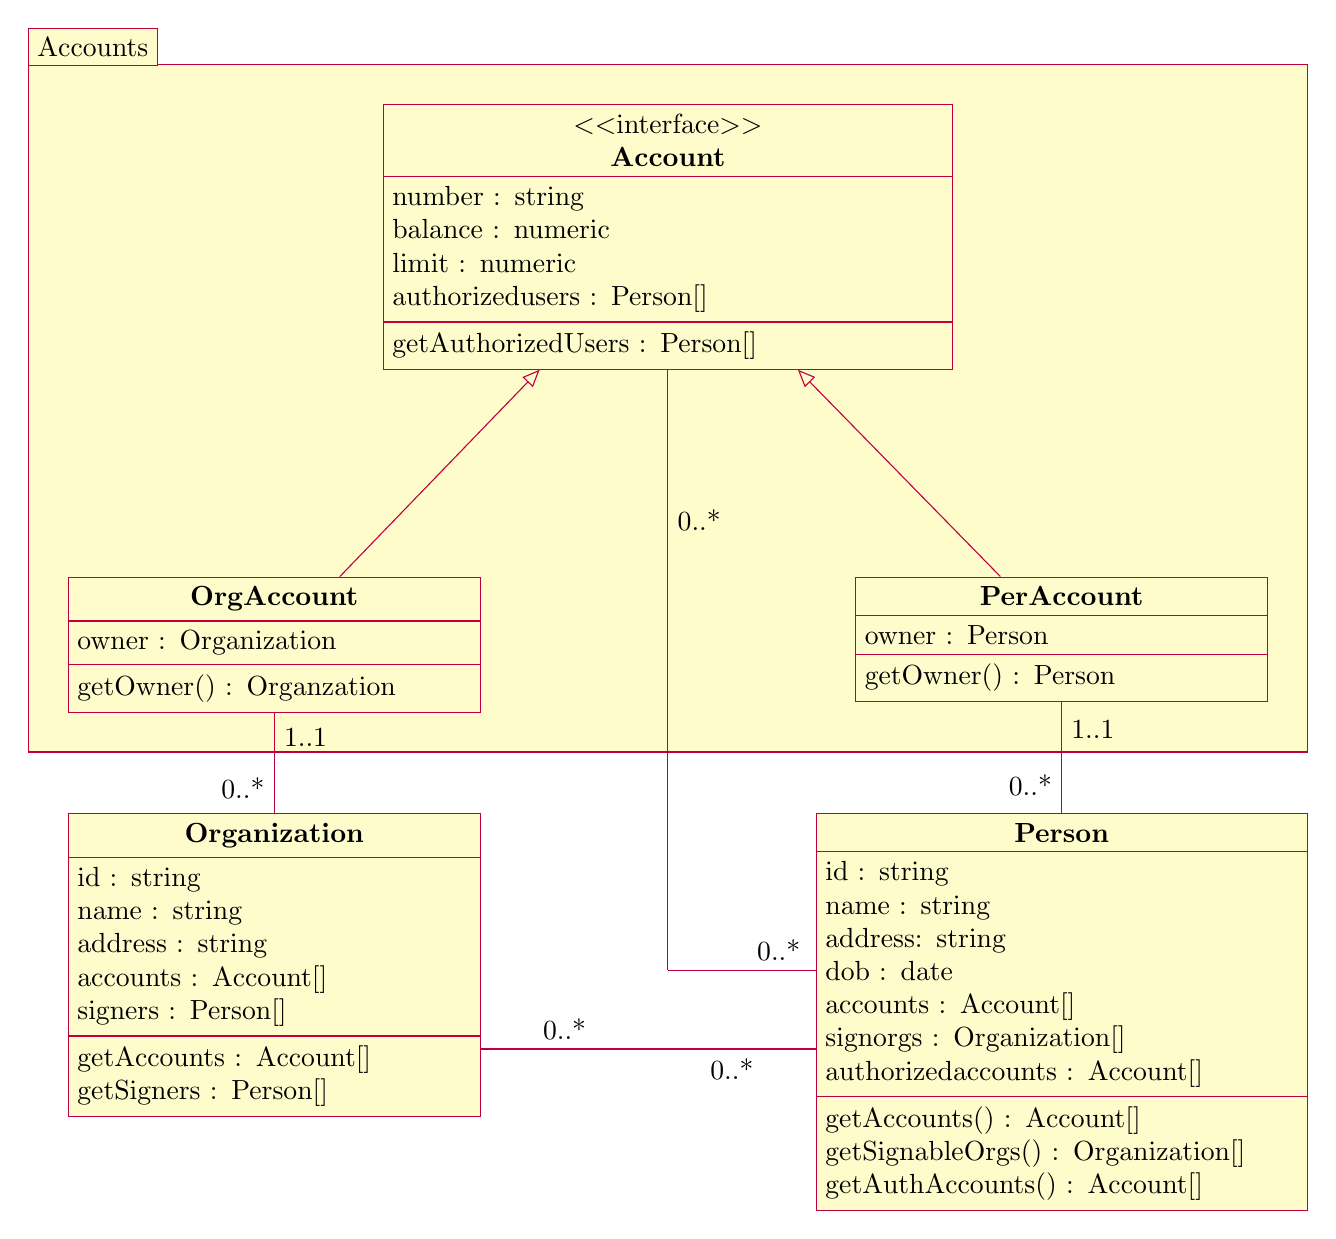
\begin{tikzpicture}
    \begin{package}{Accounts}
        \begin{interface}[text width=7cm]{Account}{0,0}
            \attribute{number : string}
            \attribute{balance : numeric}
            \attribute{limit : numeric}
            \attribute{authorizedusers : Person[]}
            \operation{getAuthorizedUsers : Person[]}
        \end{interface}

        \begin{class}[text width=5cm]{OrgAccount}{-5,-6}
            \attribute{owner : Organization}
            \inherit{Account}
            \operation{getOwner() : Organzation}
        \end{class}

        \begin{class}[text width=5cm]{PerAccount}{5,-6}
            \attribute{owner : Person}
            \inherit{Account}
            \operation{getOwner() : Person}
        \end{class}
    \end{package}
    \begin{class}[text width=5cm]{Organization}{-5,-9}
        \attribute{id : string}
        \attribute{name : string}
        \attribute{address : string}
        \attribute{accounts : Account[]}
        \attribute{signers : Person[]}
        \operation{getAccounts : Account[]}
        \operation{getSigners : Person[]}
    \end{class}
    \begin{class}[text width=6cm]{Person}{5,-9}
        \attribute{id : string}
        \attribute{name : string}
        \attribute{address: string}
        \attribute{dob : date}
        \attribute{accounts : Account[]}
        \attribute{signorgs : Organization[]}
        \attribute{authorizedaccounts : Account[]}
        \operation{getAccounts() : Account[]}
        \operation{getSignableOrgs() : Organization[]}
        \operation{getAuthAccounts() : Account[]}
    \end{class}

    %\association{OrgAccount}{}{1..1}{Organization}{0..*}{}
    \draw [umlcd style] (OrgAccount) -- (Organization) node[near start, right]{1..1} node[near end, left]{0..*};
    %\association{PerAccount}{}{1..1}{Person}{0..*}{}
    \draw [umlcd style] (PerAccount) -- (Person) node[near start, right]{1..1} node[near end, left]{0..*};

    %\association{Organization}{0..*}{}{Person}{}{0..*}

    \draw [umlcd style] (Person.west |- 5, -12) -- (Organization.east |- -5, -12) node[near start, below]{0..*} node[near end, above]{0..*};

    \draw [umlcd style] (Account) -- (0,-11) node[near start, right]{0..*};
    \draw [umlcd style] (Person.west |- 5, -11) -- (0,-11) node[near start, above]{0..*};

\end{tikzpicture}
\caption{UML diagram for CCDB}
\end{figure}


\end{document}
